\begin{figure}[!ht]
  \centering
  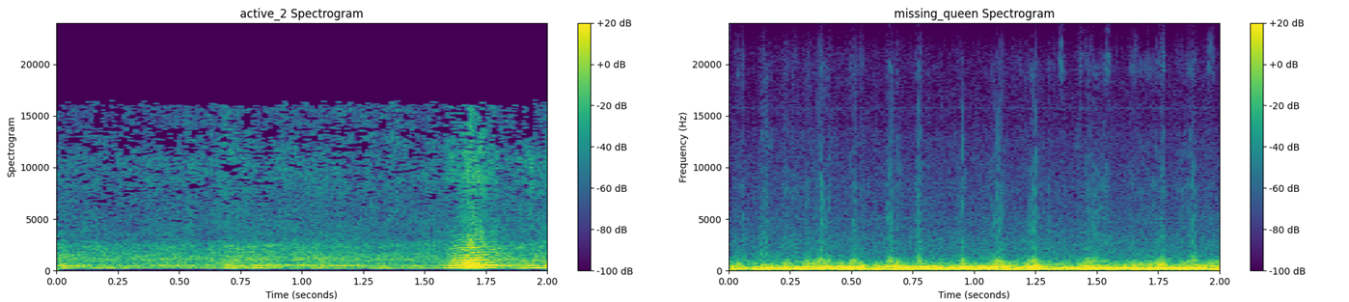
\includegraphics[width=\textwidth]{assets/cap_3/comparacion_audio.png}
  \caption{Comparación de audio.}
  \label{fig:comparacion_audio}
\end{figure}

\subsection{Características de audio}
Se describen los cálculos e implementación en Python. Se asume audio monofónico \(y\) a frecuencia de muestreo \(sr\). Para estéreo, aplicar las funciones por canal. Parámetros por defecto: \(\texttt{n\_fft}=2048\), \(\texttt{hop\_length}=512\), ventana Hann \parencite{mcfee2015librosa}.

% ======================
\subsubsection{Zero Crossing Rate (ZCR)}
\textbf{Algoritmo} \parencite{rabiner2011tasdp, tzanetakis2002musical}
\begin{enumerate}
  \item Dividir la señal continua en trozos cortos de igual tamaño llamados \emph{tramas} (por ejemplo, 2048 muestras).
  \item En cada trama, mirar el signo de la muestra actual y de la anterior. Cuando el signo cambia, contamos un cruce por cero.
  \item Sumar los cruces en la trama y normalizar por la longitud de la trama para obtener una tasa comparable entre señales.
  \item Usar la serie de tasas a lo largo del tiempo para detectar regiones ruidosas o con consonantes no sonoras.
\end{enumerate}

\textbf{Fórmula}
\[
  \text{ZCR}[t]=\frac{1}{2L}\sum_{n=1}^{L-1}\big|\operatorname{sgn}(x_t[n])-\operatorname{sgn}(x_t[n-1])\big|
\]

\textbf{Código}
\begin{lstlisting}[language=Python, label={lst:zcr_code}, caption={ZCR por tramas}]
import numpy as np
def zero_crossing_rate(y, frame_length=2048, hop_length=512):
    frames = np.lib.stride_tricks.sliding_window_view(y, frame_length)[::hop_length]
    s = np.sign(frames); s[s == 0] = 1
    return np.sum(np.abs(np.diff(s, axis=1)), axis=1)/(2*frame_length)
\end{lstlisting}

% ======================
\subsubsection{Energía}
\textbf{Algoritmo} \parencite{giannakopoulos2014intro, muller2015fmp}
\begin{enumerate}
  \item Cortar la señal en tramas.
  \item Elevar al cuadrado cada muestra de la trama para medir “cuánta señal” hay.
  \item Sumar esos cuadrados. Un valor alto indica mayor intensidad sonora en esa ventana.
\end{enumerate}

\textbf{Fórmula}
\[
  E_t = \sum_{n=1}^{L} x_t[n]^2
\]

\textbf{Código}
\begin{lstlisting}[language=Python, label={lst:energy_code}, caption={Energía por tramas}]
import librosa, numpy as np
def frame_energy(y, frame_length=2048, hop_length=512):
    f = librosa.util.frame(y, frame_length=frame_length, hop_length=hop_length)
    return np.sum(f**2, axis=0)
\end{lstlisting}

% ======================
\subsubsection{RMS (Root Mean Square)}
\textbf{Algoritmo} \parencite{oppenheim2010dsp, muller2015fmp}
\begin{enumerate}
  \item Calcular la energía de la trama.
  \item Dividir por el número de muestras para obtener una media.
  \item Tomar la raíz cuadrada para regresar a la escala de la señal. RMS es una “intensidad promedio” estable frente a picos.
\end{enumerate}

\textbf{Fórmula}
\[
  \text{RMS}_t=\sqrt{\frac{1}{L}\sum_{n=1}^{L}x_t[n]^2}
\]

\textbf{Código}
\begin{lstlisting}[language=Python, label={lst:rms_code}, caption={RMS por tramas}]
import numpy as np
def rms(y, frame_length=2048, hop_length=512):
    f = np.lib.stride_tricks.sliding_window_view(y, frame_length)[::hop_length]
    return np.sqrt(np.mean(f**2, axis=1))
\end{lstlisting}

% ======================
\subsubsection{Entropía de energía}
\textbf{Algoritmo} \parencite{peeters2004large, giannakopoulos2014intro}
\begin{enumerate}
  \item Dentro de cada trama, dividir en \(Q\) subtramas contiguas.
  \item Calcular la energía de cada subtrama y normalizar para obtener proporciones \(p_i\) que sumen 1.
  \item Calcular la entropía de Shannon de esas proporciones. Valores altos indican energía repartida; bajos, energía concentrada.
\end{enumerate}

\textbf{Fórmula}
\[
  H_t=-\sum_{i=1}^{Q}p_i\log_2 p_i,\qquad p_i=\frac{E_i}{\sum_j E_j}
\]

\textbf{Código}
\begin{lstlisting}[language=Python, label={lst:entropy_energy_code}, caption={Entropía de energía}]
import numpy as np
def energy_entropy(y, frame_length=2048, hop_length=512, n_sub=10, eps=1e-10):
    f = np.lib.stride_tricks.sliding_window_view(y, frame_length)[::hop_length]
    sub_L = frame_length//n_sub
    blocks = f[:, :sub_L*n_sub].reshape(f.shape[0], n_sub, sub_L)
    E = np.sum(blocks**2, axis=2)
    P = E/(np.sum(E, axis=1, keepdims=True)+eps)
    return -np.sum(P*np.log2(P+eps), axis=1)
\end{lstlisting}

% ======================
\subsubsection{Centroide espectral}
\textbf{Algoritmo} \parencite{tzanetakis2002musical, muller2015fmp}
\begin{enumerate}
  \item Calcular el espectro de magnitud en cada trama.
  \item Multiplicar cada magnitud por su frecuencia y promediar. Es el “centro de masa” del espectro.
\end{enumerate}

\textbf{Fórmula}
\[
  C_t=\frac{\sum_{k} f_k |X_t(f_k)|}{\sum_{k}|X_t(f_k)|}
\]

\textbf{Código}
\begin{lstlisting}[language=Python, label={lst:centroid_code}, caption={Centroide espectral}]
import librosa
def spectral_centroid(y, sr, n_fft=2048, hop_length=512):
    return librosa.feature.spectral_centroid(y=y, sr=sr, n_fft=n_fft, hop_length=hop_length)[0]
\end{lstlisting}

% ======================
\subsubsection{Dispersión espectral}
\textbf{Algoritmo} \parencite{tzanetakis2002musical, peeters2004large}
\begin{enumerate}
  \item Calcular el centroide espectral \(C_t\).
  \item Calcular la desviación estándar de las frecuencias, ponderada por la energía. Mide qué tan “ancho” es el espectro.
\end{enumerate}

\textbf{Fórmula}
\[
  \sigma_t=\sqrt{\frac{\sum_k (f_k-C_t)^2|X_t(f_k)|}{\sum_k|X_t(f_k)|}}
\]

\textbf{Código}
\begin{lstlisting}[language=Python, label={lst:spread_code}, caption={Dispersión espectral}]
import librosa
def spectral_spread(y, sr, n_fft=2048, hop_length=512):
    c = librosa.feature.spectral_centroid(y=y, sr=sr, n_fft=n_fft, hop_length=hop_length)
    return librosa.feature.spectral_bandwidth(y=y, sr=sr, n_fft=n_fft, hop_length=hop_length, centroid=c, p=2)[0]
\end{lstlisting}

% ======================
\subsubsection{Entropía espectral}
\textbf{Algoritmo} \parencite{peeters2004large, muller2015fmp}
\begin{enumerate}
  \item Calcular el espectro de magnitud y normalizarlo para que las magnitudes formen una distribución \(p_k\).
  \item Calcular la entropía de Shannon de \(p_k\). Alta entropía: espectro plano; baja entropía: energía concentrada en pocas bandas.
\end{enumerate}

\textbf{Fórmula}
\[
  H_t=-\sum_{k} p_k\log_2 p_k,\qquad p_k=\frac{|X_t(f_k)|}{\sum_{j}|X_t(f_j)|}
\]

\textbf{Código}
\begin{lstlisting}[language=Python, label={lst:spec_entropy}, caption={Entropía espectral}]
import librosa, numpy as np
def spectral_entropy(y, sr, n_fft=2048, hop_length=512, eps=1e-12):
    S = np.abs(librosa.stft(y, n_fft=n_fft, hop_length=hop_length))
    P = S/(np.sum(S, axis=0, keepdims=True)+eps)
    return -np.sum(P*np.log2(P+eps), axis=0)
\end{lstlisting}

% ======================
\subsubsection{Flujo espectral}
\textbf{Algoritmo} \parencite{foote1999novelty, muller2015fmp}
\begin{enumerate}
  \item Calcular dos espectros consecutivos y normalizarlos.
  \item Restar espectro anterior al actual. Conservar solo las diferencias positivas.
  \item Elevar al cuadrado y sumar. Valores altos indican cambios repentinos de timbre o ataque.
\end{enumerate}

\textbf{Fórmula}
\[
  \text{Flujo}_t=\sum_k\big(\max\{0, |X_t|-|X_{t-1}|\}\big)^2
\]

\textbf{Código}
\begin{lstlisting}[language=Python, label={lst:flux_code}, caption={Flujo espectral}]
import librosa, numpy as np
def spectral_flux(y, sr, n_fft=2048, hop_length=512, eps=1e-12):
    S = np.abs(librosa.stft(y, n_fft=n_fft, hop_length=hop_length))
    S /= np.sum(S, axis=0, keepdims=True)+eps
    D = np.diff(S, axis=1)
    return np.concatenate([[0.0], np.sum(np.maximum(D,0)**2, axis=0)])
\end{lstlisting}

% ======================
\subsubsection{Rolloff espectral}
\textbf{Algoritmo} \parencite{tzanetakis2002musical, peeters2004large}
\begin{enumerate}
  \item Ordenar magnitudes por frecuencia ascendente.
  \item Encontrar la frecuencia \(f_{k_c}\) donde la suma acumulada alcanza una fracción fija (por ejemplo, 85\%) de la energía total.
\end{enumerate}

\textbf{Fórmula}
\[
  \sum_{k=1}^{k_c}|X(f_k)|=\alpha\sum_{k=1}^{K}|X(f_k)|,\quad \alpha\in(0,1).
\]

\textbf{Código}
\begin{lstlisting}[language=Python, label={lst:rolloff_code}, caption={Rolloff espectral}]
import librosa
def spectral_rolloff(y, sr, n_fft=2048, hop_length=512, roll_percent=0.85):
    return librosa.feature.spectral_rolloff(y=y, sr=sr, n_fft=n_fft, hop_length=hop_length, roll_percent=roll_percent)[0]
\end{lstlisting}

% ======================
\subsubsection{MFCC (Mel Frequency Cepstral Coefficients)}
\textbf{Algoritmo} \parencite{davis1980tassp, muller2015fmp, slaney1998auditory, logan2000mfcc}
\begin{enumerate}
  \item \emph{(Opcional) Pre-énfasis}: atenuar bajas frecuencias y realzar altas con \(y[n]=x[n]-\alpha x[n-1]\) (\(\alpha\approx0.95\)). Ayuda a estabilizar el espectro.
  \item \emph{Enmarcado y ventana}: dividir en tramas de \(L\) muestras con salto \(H\). Aplicar ventana de Hann para reducir fugas espectrales.
  \item \emph{STFT y potencia}: calcular la FFT por trama y obtener espectrograma de potencias \(P_t[k]\).
  \item \emph{Banca Mel}: proyectar \(P_t[k]\) sobre \(M\) filtros triangulares \(\{H_m[k]\}\) espaciados en la escala Mel. Esto aproxima la resolución frecuencial humana.
  \item \emph{Compresión logarítmica}: \(L_t[m]=\log(E_t[m]+\varepsilon)\) con \(E_t[m]=\sum_k H_m[k]P_t[k]\). Reduce rango dinámico y aproxima la percepción.
  \item \emph{DCT-II}: aplicar DCT a \(L_t[m]\) para obtener \(c_t[i]\). Los primeros \(N\) coeficientes (típicamente 12–13) capturan la envolvente espectral. Opcionalmente omitir \(c_0\) y usar energía RMS/Log-E.
  \item \emph{(Opcional) Liftering}: suavizar la envolvente cepstral con \(S[i]\) para desacoplar lenta y rápida variación.
  \item \emph{(Opcional) Dinámicas}: calcular \(\Delta\) y \(\Delta^2\) con regresión temporal. Útiles para modelar cambios.
  \item \emph{(Recomendado) Normalización}: CMVN por señal o por conjunto para robustez entre grabaciones.
\end{enumerate}
% Sugerencias típicas: n_fft=2048, hop_length=512, n_mels=40, n_mfcc=13, lifter=22.

\textbf{Fórmulas} \parencite{davis1980tassp, muller2015fmp}
\[
  m(f)=2595\log_{10}\!\left(1+\frac{f}{700}\right),\quad
  P_t[k]=\frac{|X_t[k]|^2}{N_{\mathrm{fft}}}
\]
\[
  E_t[m]=\sum_{k=0}^{K-1} H_m[k]\;P_t[k],\qquad
  L_t[m]=\log\!\big(E_t[m]+\varepsilon\big)
\]
\[
  c_t[i]=\sum_{m=0}^{M-1} L_t[m]\cos\!\Big(\frac{\pi i}{M}\big(m+\tfrac12\big)\Big),\quad i=0,\dots,N-1
\]
\[
  \tilde c_t[i]=\Big(1+\frac{L_c}{2}\sin\frac{\pi i}{L_c}\Big)c_t[i]\quad\text{(liftering, \(L_c\approx22\))}
\]
\[
  \Delta c_t[i]=\frac{\sum_{n=1}^{N_d}n\big(c_{t+n}[i]-c_{t-n}[i]\big)}{2\sum_{n=1}^{N_d}n^2}\quad\text{(típico \(N_d=2\))}
\]

\textbf{Código} \parencite{davis1980tassp, muller2015fmp}
\begin{lstlisting}[language=Python, label={lst:mfcc_code}, caption={MFCC básicos (librosa)}]
import numpy as np
import librosa

def mfcc_13(y, sr, n_fft=2048, hop_length=512, n_mels=40, n_mfcc=13):
    return librosa.feature.mfcc(y=y, sr=sr, n_fft=n_fft,
                                hop_length=hop_length,
                                n_mels=n_mels, n_mfcc=n_mfcc)
\end{lstlisting}

\begin{lstlisting}[language=Python, label={lst:mfcc_full_code}, caption={Pipeline explícito: pre-énfasis, Mel, log, DCT, deltas y liftering}]
import numpy as np
import librosa

def mfcc_full(y, sr, n_fft=2048, hop_length=512,
              n_mels=40, n_mfcc=13, pre_emph=0.97,
              lifter=22, use_c0=False):
    # 1) Pre-énfasis
    if pre_emph is not None and 0 < pre_emph < 1:
        y = np.append(y[0], y[1:] - pre_emph * y[:-1])

    # 2) Potencia
    S = np.abs(librosa.stft(y, n_fft=n_fft, hop_length=hop_length, window='hann'))**2

    # 3) Banca Mel y energías
    mel_fb = librosa.filters.mel(sr=sr, n_fft=n_fft, n_mels=n_mels, norm='slaney')
    E = np.dot(mel_fb, S)  # (n_mels, n_frames)

    # 4) Log-energías con epsilon
    eps = 1e-10
    L = np.log(E + eps)

    # 5) DCT-II (usar rutina de librosa para asegurar ortonormalidad)
    #    Esto replica librosa.feature.mfcc pero partiendo de L ya calculado:
    mfcc = librosa.feature.mfcc(S=librosa.power_to_db(E, ref=np.max),
                                n_mfcc=n_mfcc)  # equivalente y estable

    # 6) Omitir c0 si se desea usar energía por separado
    if not use_c0 and mfcc.shape[0] >= 1:
        mfcc = mfcc[1:n_mfcc+1, :]

    # 7) Liftering (cepstral)
    if lifter is not None and lifter > 0:
        Q = mfcc.shape[0]
        lift = 1 + (lifter/2.0) * np.sin(np.pi * np.arange(Q) / lifter)
        mfcc = (lift[:, None]) * mfcc

    # 8) Dinámicas
    d1 = librosa.feature.delta(mfcc, order=1, width=9, mode='interp')
    d2 = librosa.feature.delta(mfcc, order=2, width=9, mode='interp')

    # 9) CMVN por coeficiente (opcional)
    def cmvn(X, eps=1e-8):
        mu = X.mean(axis=1, keepdims=True)
        sd = X.std(axis=1, keepdims=True)
        return (X - mu) / (sd + eps)

    return cmvn(mfcc), cmvn(d1), cmvn(d2)
\end{lstlisting}

% Notas: Ajustar n_mels y n_mfcc según el dominio (zumbido de colmena suele concentrar energía en bandas medias-bajas).

